\section*{Результаты измерений}

\subsection*{Определение фокусного расстояния тонкой положительной линзы с помощью метода Аббе}

Результаты вычислений фокусных расстояний для разных экспериментальных измерений представлены на рисунке:

\begin{figure}[H]
	\centering
	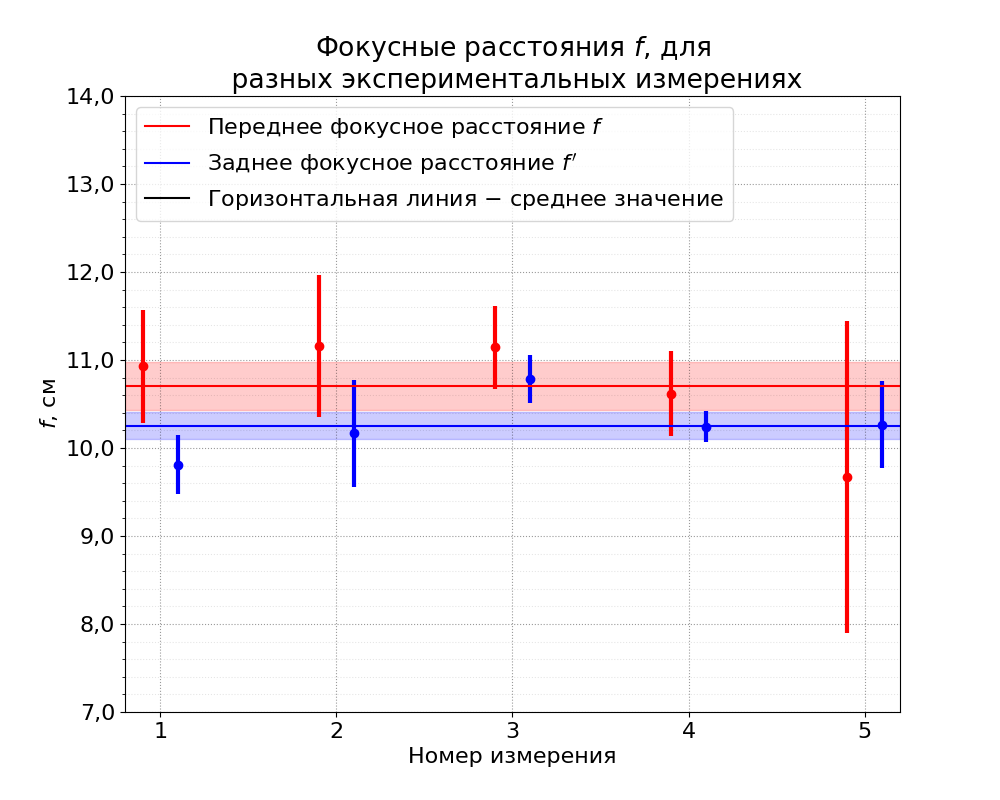
\includegraphics[width=0.6\textwidth]{../Графики/abbe_f.png}
\end{figure}

Итоговое переднее и заднее фокусные расстояния оценим как среднее:\\
Переднее фокусное расстояние $f = 10,7 \pm 0,3$ \\
Заднее фокусное расстояние $f' = 10,3 \pm 0,2$.

Случайную погрешность измерения среднего значения оценим по формуле:
$$
\sigma_{ср} = \sqrt{\frac{1}{n(n-1)} \sum\limits_{i = 1}^n (x_i - x_{ср})^2}
$$

Для тонкой линзы переднее и заднее фокусные расстояния равны. Толщину линзы оценим как разность фокусных расстояний $\delta \sim 5 \mm$. Так как $\delta$ малая величина, то итоговое фокусное расстояние оценим как среднее переднего и заднего:
$f = 10,5 \pm 0,3$. \\
Оптическая сила $D = 9,5 \pm 0,2 \dptr$.

\subsection*{Определение фокусного расстояния тонкой положительной линзы с помощью метода Бесселя}

В результате экспериментальных наблюдений было установлено:
\begin{enumerate}
	\item При небольшом расстоянии $L < 60 \cm$ от предмета до оптической системы чёткость изображения слабо зависит от яркости и размера диафрагмы. При большей яркости предмета изображение лучше различимо, оно более контрастное.
	
	\item При больших расстояниях $L > 60 \cm$. Изображение неразличимо из-за того, что оно слишком маленькое. Фокусировка производилась при слабо открытой диафрагме, при наибольшей яркости. Расстояние устанавливалось так, чтобы изображение имело наименьший размер, то есть его границы были резкими. При небольших расстояниях $L$ было установлено, что чёткое изображение при большой диафрагме и резкое пятно при малой диафрагме наблюдаются при разном положении экрана, но как будет видно при обработке данных из-за большого расстояния $L$ отклонение результатов лежит в пределах погрешности.
\end{enumerate}

Результаты вычислений фокусных расстояний для разных экспериментальных измерений представлены на рисунке:

\begin{figure}[H]
	\centering
	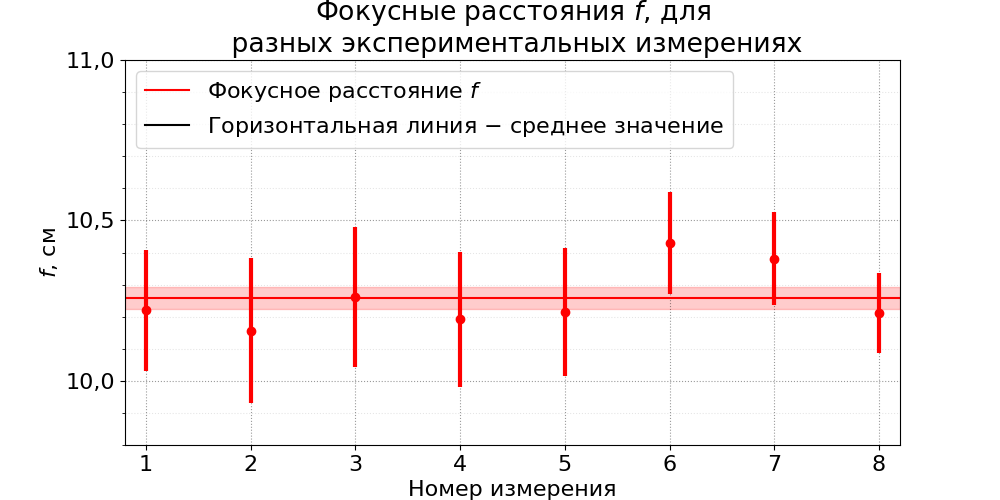
\includegraphics[width=0.6\textwidth]{../Графики/bessel_full_f.png}
\end{figure}

При вычислениях применялась приближённая формула, где толщина линзы оценивалась как $\delta = 5 \mm$.

В данном методе предполагалось, что переднее и заднее фокусные расстояния равны. Итоговое среднее значение фокусного расстояния: \\
$f = 10,25 \pm 0,03 \cm$ \\
Оптическая сила $D = 9,80 \pm 0,03 \dptr$.

\subsection*{Определение фокусного расстояния тонкой отрицательной линзы с помощью метода Бесселя}

Результаты вычислений фокусных расстояний для разных экспериментальных измерений представлены на рисунке:

\begin{figure}[H]
	\centering
	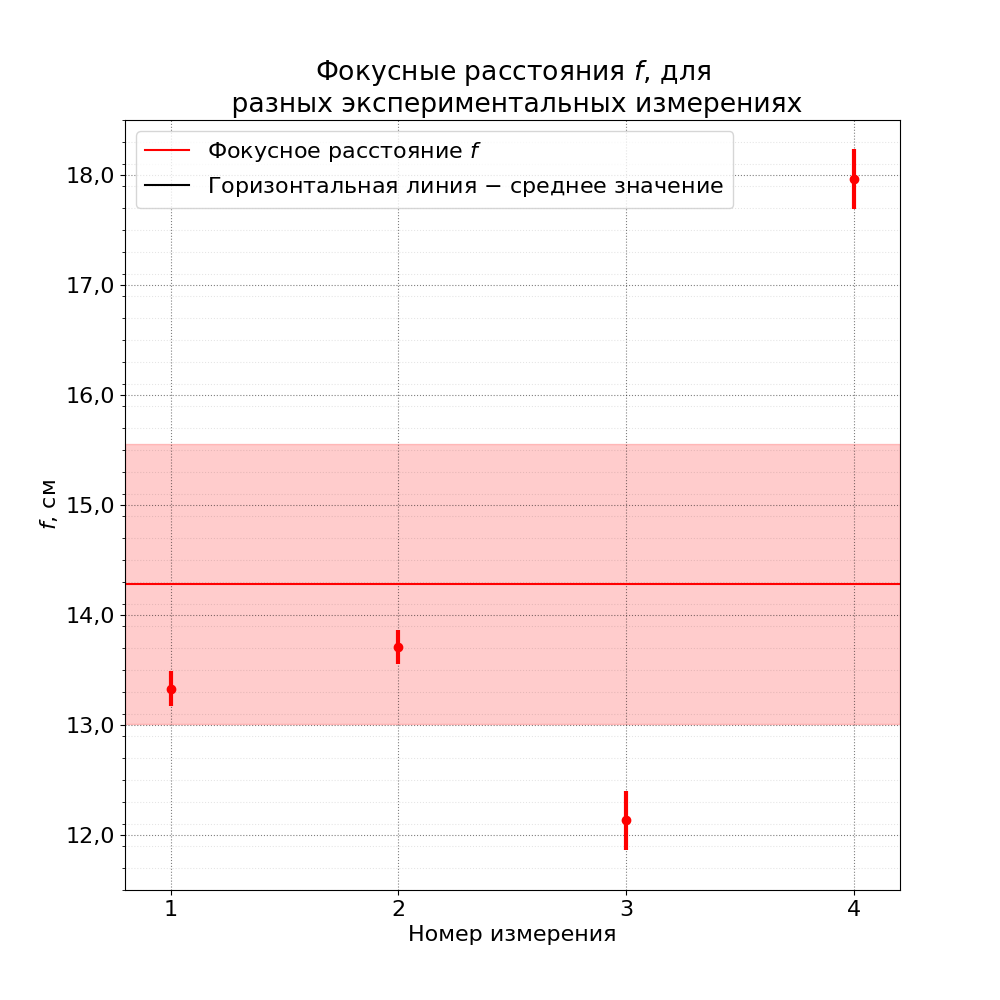
\includegraphics[width=0.6\textwidth]{../Графики/otr_full_f.png}
\end{figure}

Для более точного определения фокусного расстояния рассеивающей линзы нужно проводить дополнительные измерения. Но так как такой возможности нет, то проанализируем имеющиеся данные. Экспериментальная точка 4 выпадает из общей зависимости, отбросим её.

\begin{figure}[H]
	\centering
	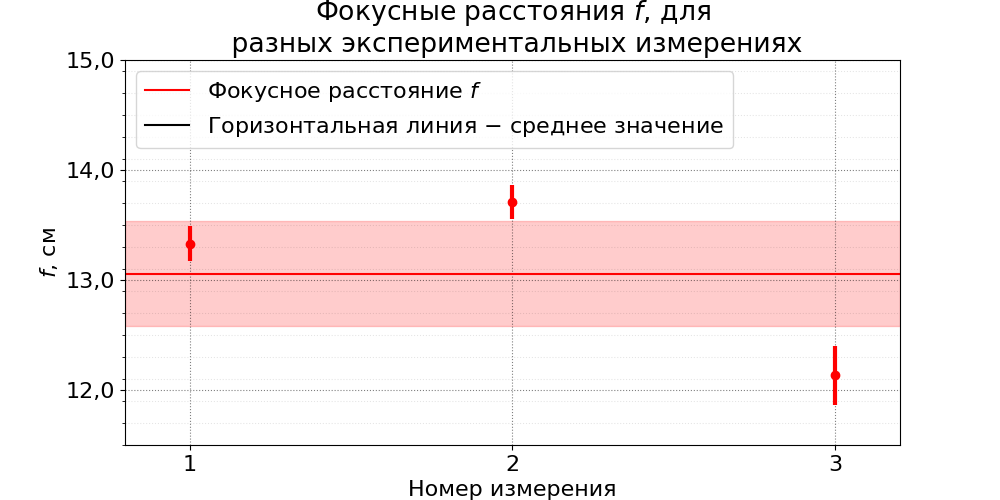
\includegraphics[width=0.6\textwidth]{../Графики/otr_f.png}
\end{figure}

Итоговое среднее значение фокусного расстояния: \\
$f = -13,1 \pm 0,5 \cm$ \\
Оптическая сила $D = -7,6 \pm 0,3 \dptr$.

\subsection*{Определение фокусного расстояния тонких положительной и отрицательной линз с помощью оптической трубы}

Повторные измерения 

С помощью оптической трубы для положительной линзы были измерены фокусные расстояния тонких линзы:

Положительная линза №1: \\
Передний фокус $f = 9,1 \pm 0,1 \cm$ \\
Задний фокус $f = 9,4 \pm 0,1 \cm$.

Положительная линза №2: \\
Передний фокус $f = 11,4 \pm 0,1 \cm$ \\
Задний фокус $f = 11,5 \pm 0,1 \cm$.

Отрицательная линза: \\
Передний фокус $f = -15,0 \pm 0,1 \cm$ \\
Задний фокус $f = -14,7 \pm 0,1 \cm$.

Измеренные фокусные расстояния слабо отличаются, итоговое фокусное расстояние в приближении, что линзы тонкие, оценим как среднее.

Положительная линза №1: \\
$f = 9,3 \pm 0,1 \cm$. \\
Оптическая сила $D = 10,8 \pm 0,1 \dptr$.

Положительная линза №2: \\
$f = 11,5 \pm 0,1 \cm$. \\
Оптическая сила $D = 8,7 \pm 0,1 \dptr$.

Отрицательная линза: \\
$f = -14,9 \pm 0,1 \cm$. \\
Оптическая сила $D = -6,7 \pm 0,1 \dptr$.

\subsection*{Определение фокусного расстояния тонких положительной и отрицательной линз с помощью оптической трубы}

Фокусные расстояния линз: 
\begin{table}[]
	\begin{tabular}{ccc}
		№ Линзы & F(cм) & D(дптр) \\
		1       & 10.3  & 9.75    \\
		2       & 12.8  & 7.81    \\
		3       & 7.0   & 14.29   \\
		4       & -14.8 & -6.76  
	\end{tabular}
	\caption{}
\end{table}

Определение фокусного расстояния системы двух линз методом Аббе:
\textbf{F = 6.38}\\

Определение фокусного расстояния системы двух линз с помощью зрительной трубы:
\begin{table}[]
	\begin{tabular}{cc}
		F1    & F2      \\
		4.6 см & 3.8 см
	\end{tabular}
	\caption{F1 - фокус при конфигурации линз "12", F2 - при "21"}
\end{table}